\section{Cyclotron mass}
For small magnetic fields and therefore $E_\text{F}>>\hbar\omega_\text{c}$, "within the framework of self-consistent Born approximation" \cite{Tasksheet}, 
the cyclotron mass $m_\text{c}$ can be calculated according to \cite{Ando}.\\
The longitudinal conductance $\sigma_\text{xx}$ \cite{Ando} can be rewritten into eq.\,\ref{eq:sigmaxxCyclotron}
\begin{align}
    \sigma_\text{xx}(B) = \sigma_\text{background}\cdot\left(1-A(B,T,\tau)\cos{\left(\frac{2\pi E_\text{F}}{\hbar\omega}\right)}\right)
    \label{sigmaxxCyclotron}
\end{align}
with $\sigma_\text{background}=\frac{ne^2\tau}{m_\text{c}(1+\omega_\text{c}^2\tau^2)}$, $A(B,T,\tau)$ as the amplitude function and $E_\text{F}$ as the Fermi energy. 
To isolate the oscillations from the background, $\sigma_\text{background}$ is fittet by eq.\,\ref{eq:fit}
\begin{align}
    \sigma_\text{background}(B) = \frac{a}{1+bB^2}
    \label{eq:fit}
\end{align}
with $a$ and $b$ as fit parameters. The fit of $\sigma_\text{background}$ and $\sigma_\text{xx}$ is shown in fig.\,\ref{fig:fitCyclotron}.
\begin{figure}[h]
    \centering
    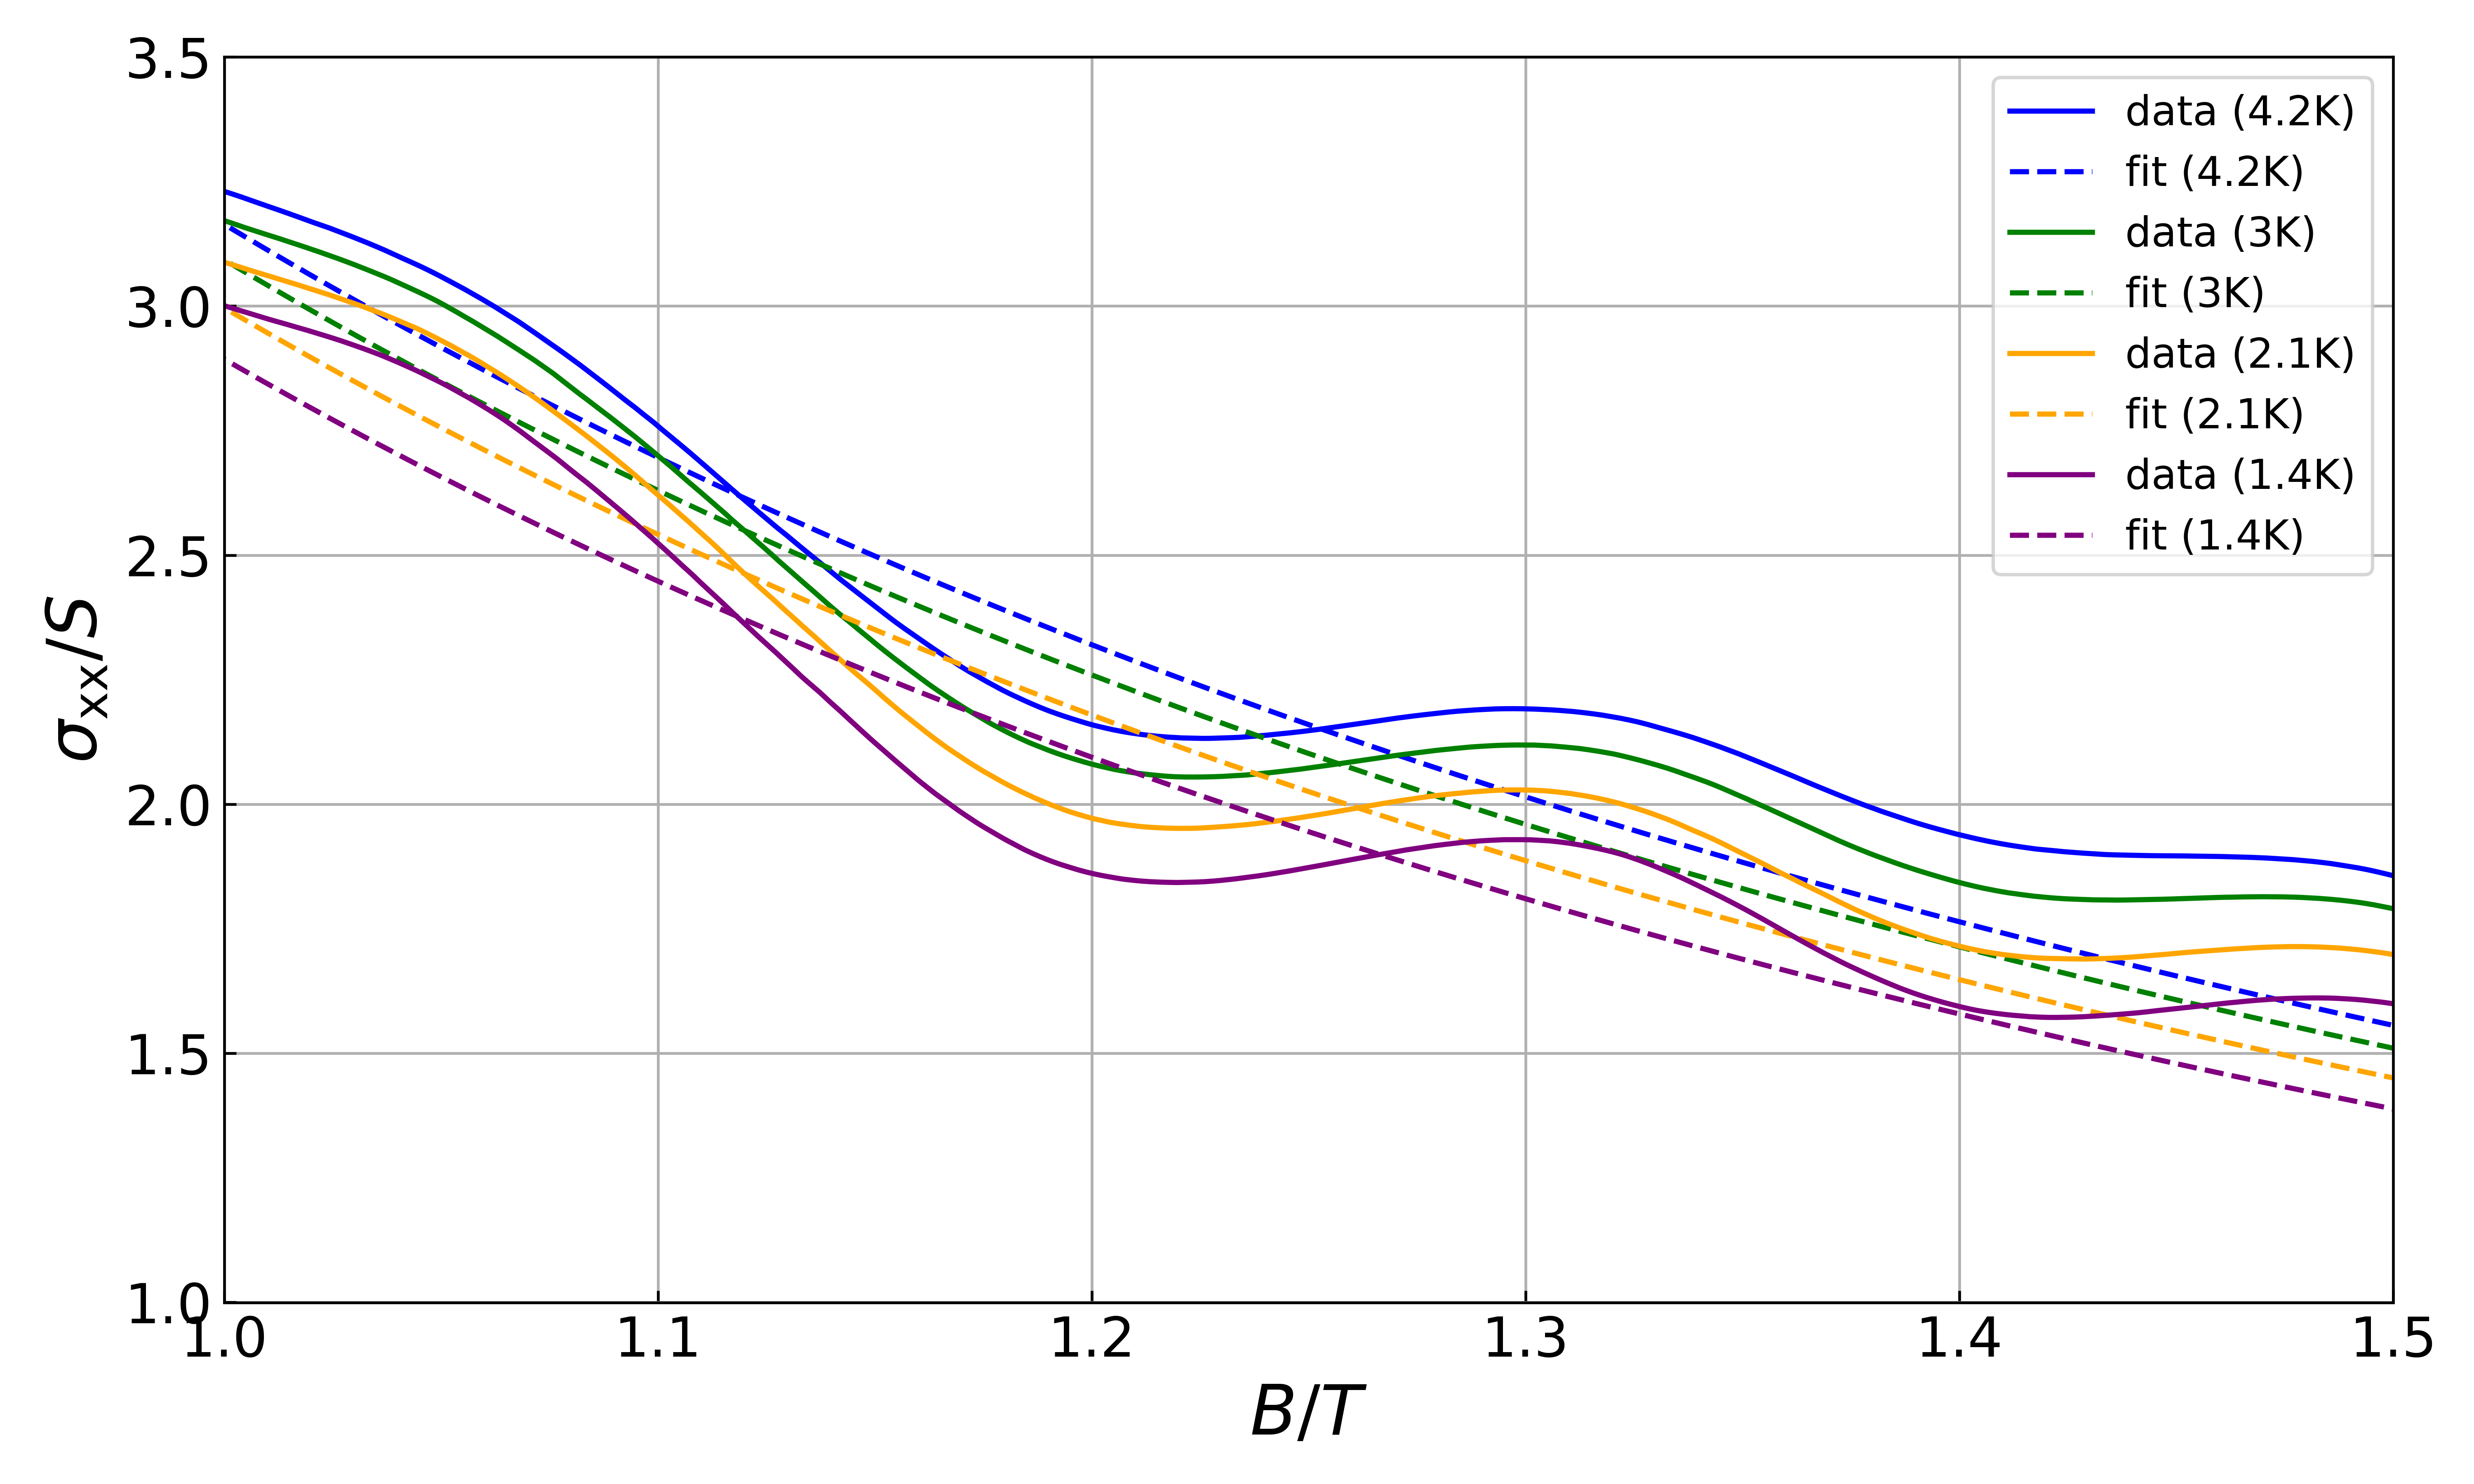
\includegraphics[width=0.45\textwidth]{../Images/sigmaWithFit.png}
    \caption{Examplary fit of the background of the longitudinal conductance $\sigma_\text{xx}$ at various temperatures. 
    The shown range of the plot is picked because of good visibility of the fit. The total fit is done for a wider range ($0.5\,\text{T}$ to $1.5\,\text{T}$) like stated in the text.}
    \label{fig:fitCyclotron}
\end{figure}
The fit is done for magnetic fields in the range of $0.5\,\text{T}$ to $1.5\,\text{T}$, 
where the magnetic field is still small enough so that eq.\,\ref{sigmaxxCyclotron} holds.
By deviding $\sigma_\text{xx}$ by $\sigma_\text{background}$ and adding a $1$, the oscillations can be isolated which can
be seen in fig.\,\ref{fig:oscillationsCyclotron}.
\begin{figure}[h]
    \centering
    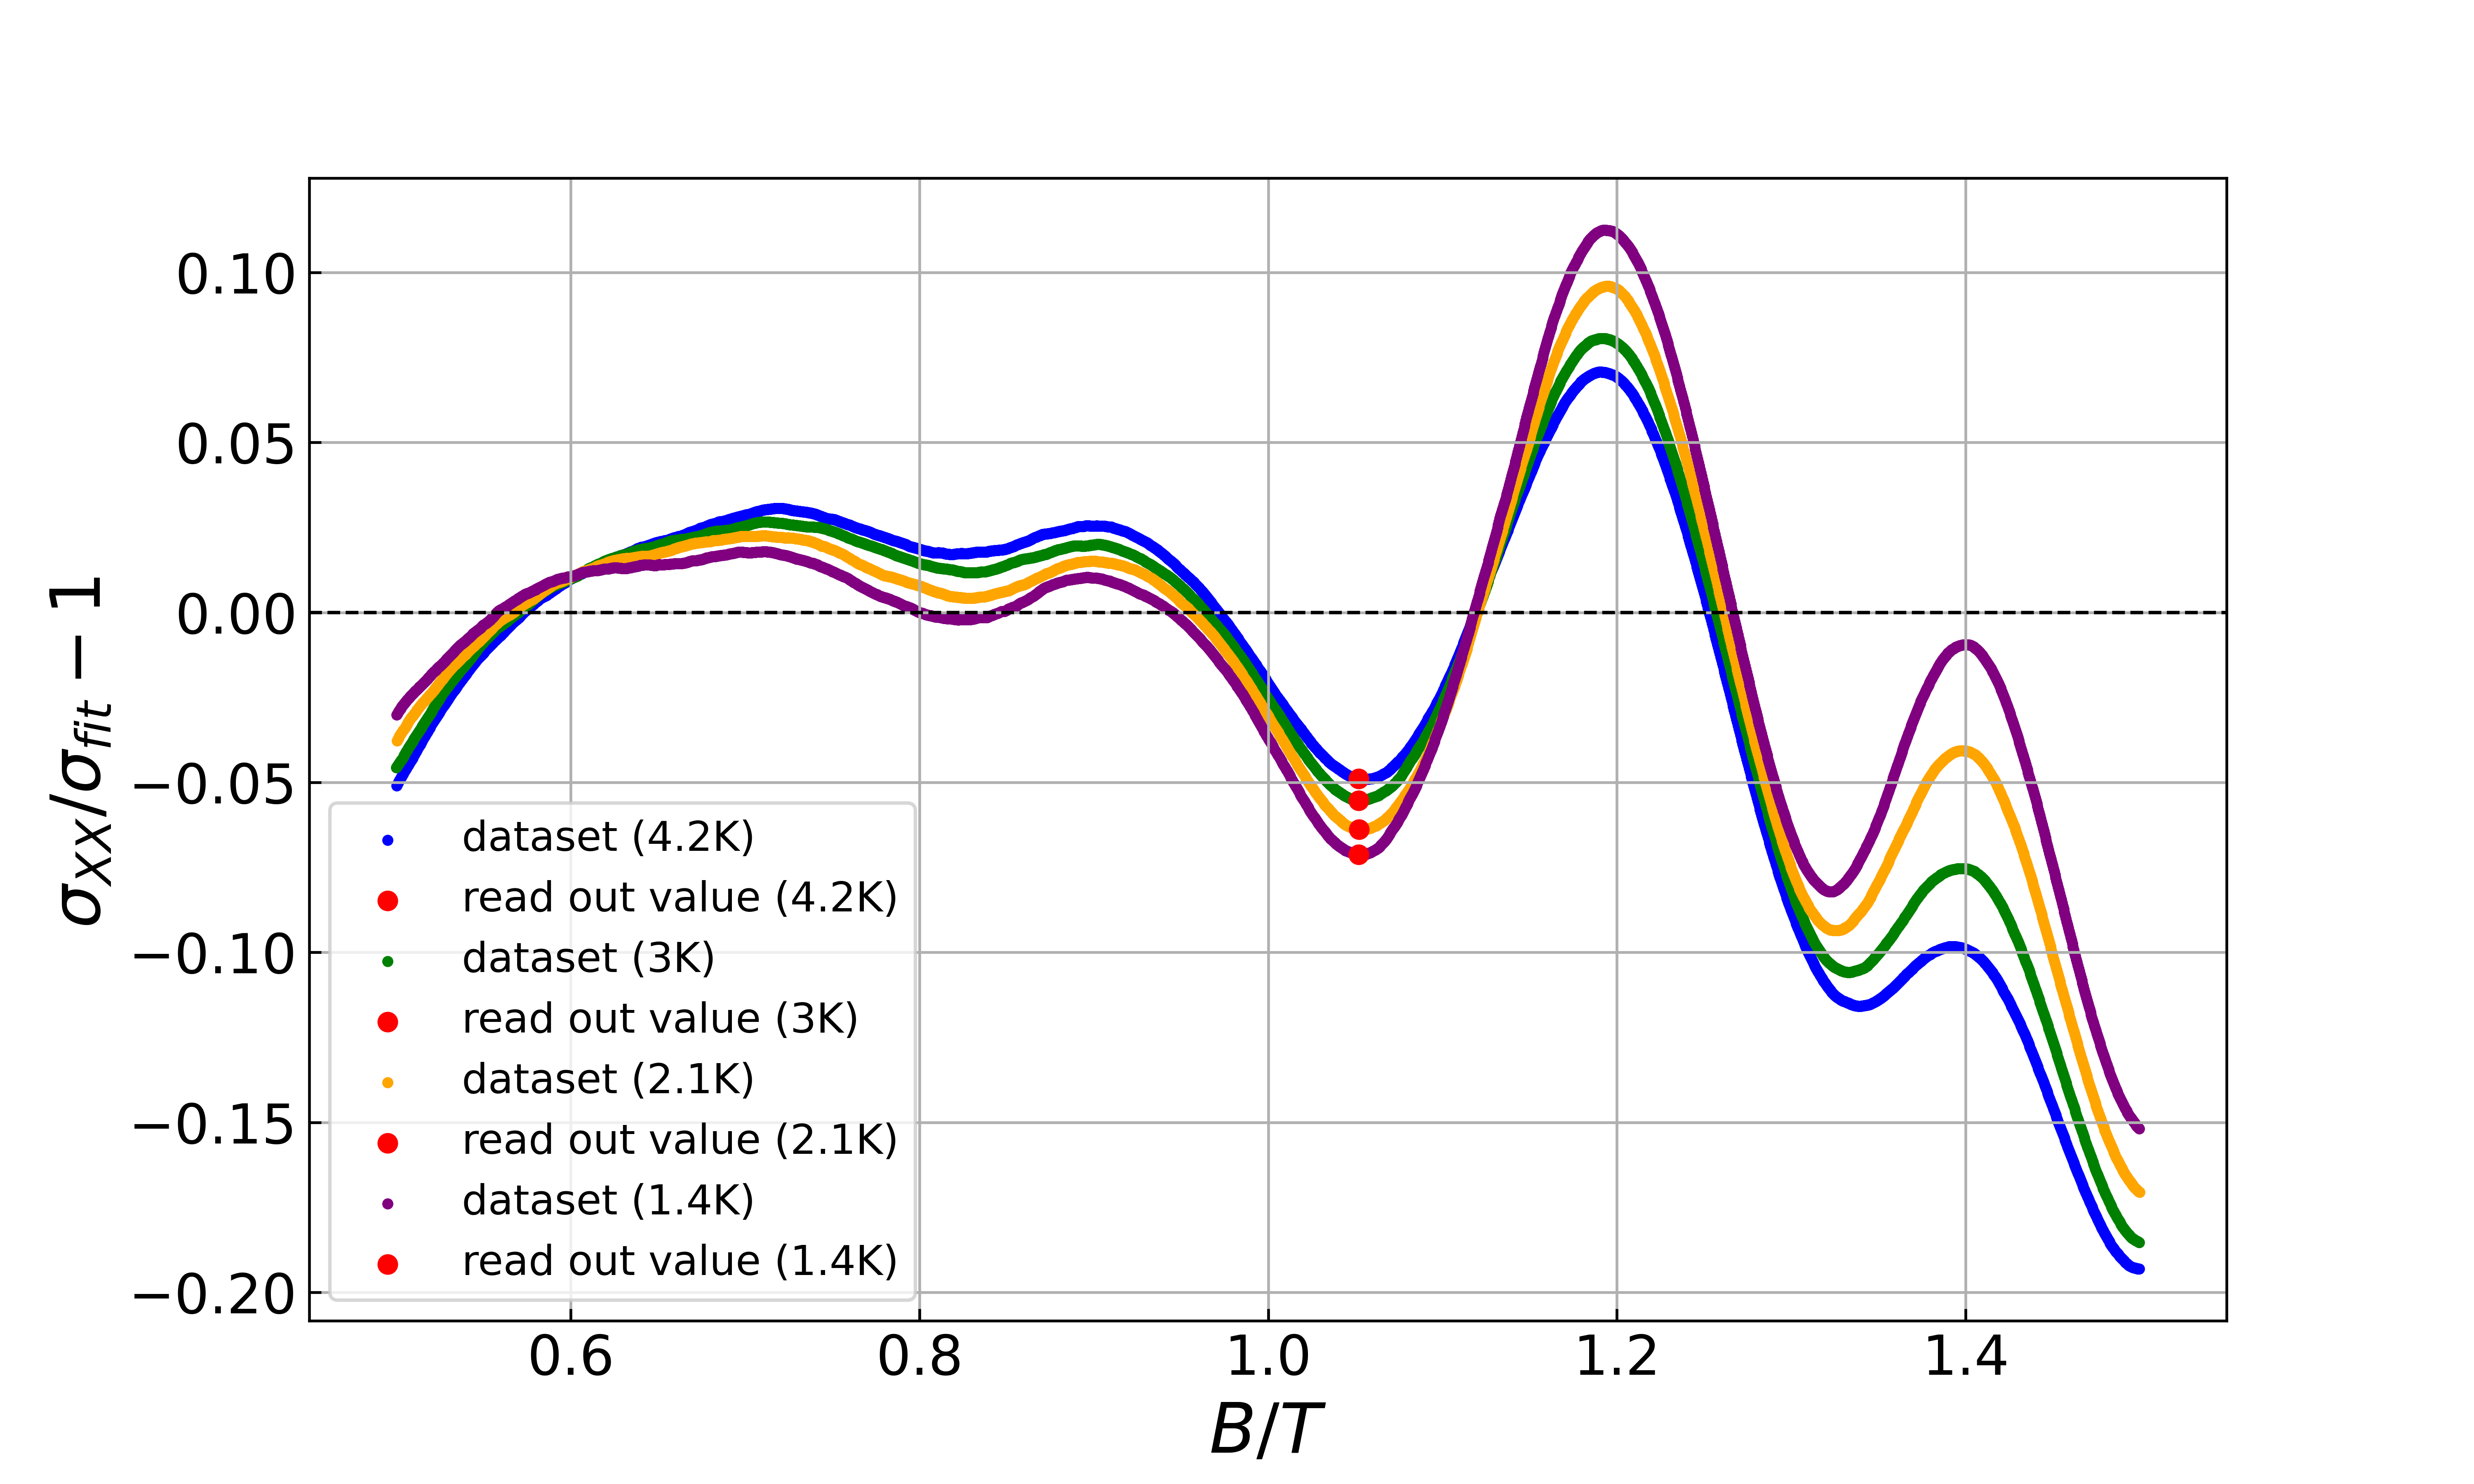
\includegraphics[width=0.45\textwidth]{../Images/reducedSigma.png}
    \caption{Isolated scillations of the longitudinal conductance $\sigma_\text{xx}$ at various temperatures.}
    \label{fig:oscillationsCyclotron}
\end{figure}
This is in accordance with eq.\,\ref{sigmaxxCyclotron}, which then simplifies to eq.\,\ref{eq:onlyOscillation}
\begin{align}
    \sigma_\text{xx}(B) = A(B,T,\tau)\cdot\cos{\left(\frac{2\pi E_\text{F}}{\hbar\omega}\right)}
    \label{eq:onlyOscillation}
\end{align}
Like shown in fig.\,\ref{eq:onlyOscillation}, the amplitudes of the first pronounced oscillation for
the temperatures ($1.4\,K$,$3\,K$) and ($2.1\,K$,$4.2\,K$) are read out as pairs ($A(T_1)$,$A(T_2)$).
The chosen oscillation is small enough that with $A_\text{ratio}=\frac{A(T_1)}{A(T_2)}$ eq.\,\ref{mc/me} is valid \cite{Tasksheet}.
\begin{align}
    \frac{m_\text{c}}{m_\text{e}}=\frac{\hbar eB}{m_\text{e}\pi^2k_\text{B}T_1}\text{arcosh}\left(A_\text{ratio}\right)
\end{align}
With eq.\,\ref{mc/me} the cyclotron mass $m_\text{c}$ can be calculated. The results are shown in tab.\,\ref{tab:cyclotronMass}.
\begin{table}[h]
    \centering
    \begin{tabular}{c|c}
        \hline\hline
        $m_{\text{c}1.4\text{K},3\text{K}}$ & $m_{\text{c}2.1\text{K},4.2\text{K}}$ \\\hline
        $(\csname cyclotron15\endcsname)$\cdot$10^{-2}m_\text{e}$& $(\csname cyclotron21\endcsname)$\cdot$10^{-2}m_\text{e}$ \\
        \hline\hline
    \end{tabular}
\end{table}
The literature expects cyclotron masses of $m_\text{c}= 0.026m_\text{e}$ to $m_\text{c}= 0.048m_\text{e}$ \cite{Xhang}.
The determined value for the $1.4\,K$ and $3\,K$ pair is in the range of the literature value, whereas the value for the $2.1\,K$ and $4.2\,K$ pair is slightly lower
but still agrees within its errors.
As seen in fig.\,\ref{fig:onlyOscillation}, the read out of the amplitude is very subjective and more error prown than the reading of the magnetic field.
Additionally, some uncertainty regarding the fit of the background is included in the error of the amplitude.
On this basis an error of $10\%$ is assumed for the amplitude and $1\%$ for the magnetic field.
The errors are calculated with gaussian error propagation for the error of the amplitude and the corresponding magnetic field.